\section{Complessi}
Ragionamenti di questo tipo hanno portato alla creazione di un nuovo campo numerico: quello dei \textbf{complessi} (insieme $\C$).

\begin{defin}
	Si chiama insieme $\C$ dei numeri complessi l'insieme $\R^2$ (ovvero $\R\times\R$) e numero complesso ciascun elemento di $\C$, ossia una coppia ordinata di numeri reali.
\end{defin}
Per convenzione e semplicità il numero complesso $z$, che in quanto elemento di un prodotto cartesiano dovrebbe essere espresso con una coppia di coordinate nella forma $(a;b)$, si esprime invece nella forma
\[
	z = a + bi
\]
Il numero $a$ si chiama parte reale del numero complesso e si indica con $\re z$, il numero $b$ si chiama parte immaginaria del numero complesso e si indica con $\im z$. La parte reale e quella immaginaria si possono omettere quando rispettivamente $a$ e $b$ sono uguali a $0$.

\begin{defin}
	Due numeri complessi $z$ e $w$ si dicono:
	\begin{itemize}
		\item \emph{Uguali} se $\re z=\re w\land\im z=\im w$
		\item \emph{Coniugati} se $\re z=\re w\land\im z=-\im w$. Il coniugato di un numero $z$ si indica con $\bar z$
		\item \emph{Opposti} se $\re z=-\re w\land\im z=-\im w$
	\end{itemize}
	Inoltre si definisce modulo di un numero complesso $z$ e si indica con $\abs{z}$ il numero
	\[
		\sqrt{a^2+b^2}
	\]
\end{defin}


\subsection{Operazioni in \texorpdfstring{$\C$}{C}}
In $\C$ appare una proprietà del tutto nuova:
\[
	i^2=-1
\]
Presa in considerazione tale proprietà, in $\C$ si definiscono le seguenti operazioni, analoghe a ciò che avverrebbe nei reali considerando $a+bi$ un binomio nella variabile $i$:
\begin{defin}{Addizione di complessi}
	\[
		(a+bi)+(c+di)=(a+c)+(b+d)i
	\]
\end{defin}
\begin{defin}{Moltiplicazione di complessi}
	\begin{gather*}
		(a+bi)(c+di)=\\
		=ac+adi+bci+bdi^2=\\
		=ac+(ad+bc)i+bd(-1)=\\
		=(ac-bd)+(ad+bc)i
	\end{gather*}
\end{defin}

\subsubsection{Proprietà}
Nell'insieme $\C$ le operazioni godono di proprietà analoghe a quelle che valgono in $\R$.
\begin{description}
	\item[Addizione] L'addizione è commutativa e associativa, inoltre
		\begin{itemize}
			\item ha come elemento neutro il numero complesso $0+0i$ (o $0$)
			\item ogni numero complesso $a+bi$ ammette come opposto il numero $-a-bi$
		\end{itemize}
	\item[Moltiplicazione] La moltiplicazione è commutativa, associativa e distributiva rispetto all'addizione, inoltre
		\begin{itemize}
			\item ha come elemento neutro il numero complesso $1+0i$ (o $1$)
			\item ogni numero complesso $a+bi$, diverso da $0$, ammette come reciproco il numero $\dfrac{\bar z}{\abs{z}^2}=\dfrac{a-bi}{a^2+b^2}$, ossia il loro prodotto è uguale a $1$:
			      \begin{gather*}
				      ( a + bi ) \left( \frac{a - bi}{a^2 + b^2} \right) = \\
				      = \frac{a^2 - abi + abi + b^2}{a^2 + b^2} = \\
				      = \frac{a^2 + b^2}{a^2 + b^2} = 1
			      \end{gather*}
		\end{itemize}
\end{description}

\subsubsection{Proprietà del coniugio e del modulo}
L'operazione di coniugio, cioè di determinazione del coniugato di un numero complesso, e quella di modulo hanno alcune proprietà:
\begin{prop}
	Dati due numeri complessi $z=a+bi$ e $w=c+di$, valgono le seguenti proprietà:
	\begin{align}
		\label{compl:comouno}
		\bullet~ & \bar z=z\iff z\in\R                                  \\
		\label{compl:comodue}
		\bullet~ & \bar z=-z\iff z\in i\R                               \\
		\label{compl:comotre}
		\bullet~ & \overline{z+w}=\bar z+\bar w                         \\
		\label{compl:comoquattro}
		\bullet~ & \overline{z*w}=\bar z\bar w                          \\
		\label{compl:comocinque}
		\bullet~ & \abs{\bar z}=\abs{z}                                 \\
		\label{compl:comosei}
		\bullet~ & \abs{zw}=\abs{z}\abs{w}                              \\
		\label{compl:comosette}
		\bullet~ & \overline{\left(\frac{1}{z}\right)}=\frac{1}{\bar z} \\
		\label{compl:comootto}
		\bullet~ & z*\bar z=\abs{z}^2
	\end{align}
\end{prop}

% TODO: riformattare in un unico proof con un itemize/description con i ref ai vari punti
\begin{proof}[\ref{compl:comouno}]
	\begin{gather*}
		\bar z = z \iff \re \bar z = \re z \land \im \bar z = \im z \\
		a = a \quad \forall a \in \R \qquad b = -b \iff b = 0
	\end{gather*}
\end{proof}
\begin{proof}[\ref{compl:comodue}]
	Analogo alla precedente.
\end{proof}

\begin{proof}[\ref{compl:comotre}]
	\begin{equation*}
		\overline{z+w}=\overline{a+bi+c+di}=\overline{(a+c)+(b+d)i}=(a+c)-(b+d)i\\
	\end{equation*}
	\center al contempo:
	\begin{equation*}
		\bar z+\bar w= \overline{a+bi}+\overline{c+di}=a-bi+c-di=(a+c)-(b+d)i
	\end{equation*}
\end{proof}
\begin{proof}[\ref{compl:comoquattro}]
	\begin{equation*}
		\overline{z*w}=\overline{(a+bi)(c+di)}=\overline{(ac-bd)+(bc+ad)i}=(ac-bd)-(bc+ad)i\\
	\end{equation*}
	\center al contempo:
	\begin{equation*}
		\bar z*\bar w=\overline{a+bi}*\overline{c+di}=(a-bi)(c-di)=(ac-bd)-(bc+ad)i
	\end{equation*}
\end{proof}
\begin{proof}[\ref{compl:comocinque}]
	\begin{equation*}
		\abs{z} = \sqrt{a^2 + b^2} \\
	\end{equation*}
	\center al contempo:
	\begin{equation*}
		\abs{\bar z} = \sqrt{a^2 + ( -b )^2} = \sqrt{a^2 + b^2}
	\end{equation*}
\end{proof}
\begin{proof}[\ref{compl:comosei}]
	\begin{align*}
		\abs{zw} & = \sqrt{(ac-bd)^2+(bc+ad)^2} =                   \\
		         & = \sqrt{a^2c^2-2abcd+b^2d^2+b^2c^2+2abcd+a^2d^2} \\
	\end{align*}
	\center al contempo:
	\begin{align*}
		\abs{z}\abs{w} & = \sqrt{a^2+b^2}\sqrt{c^2+d^2}      \\
		               & =\sqrt{a^2c^2+a^2d^2+b^2c^2+b^2d^2}
	\end{align*}
\end{proof}
\begin{proof}[\ref{compl:comosette}]
	\begin{equation*}
		\overline{\left(\frac{1}{z}\right)}=\overline{\left(\frac{1}{a}+\frac{1}{b}i\right)}=\frac{1}{a}-\frac{1}{b}i\\
	\end{equation*}
	\center al contempo:
	\begin{equation*}
		\frac{1}{\bar z}=\frac{1}{\overline{a+bi}}=\frac{1}{a-bi}=\frac{1}{a}-\frac{1}{b}i
	\end{equation*}
\end{proof}
\begin{proof}[\ref{compl:comootto}]
	\begin{gather*}
		z*\bar z=(a+bi)(a-bi)=a^2-bi^2=a^2+b^2=\left(\sqrt{a^2+b^2}\right)^2=\abs{z}^2
	\end{gather*}
\end{proof}


\subsection{Rappresentazione grafica}
La definizione di numero complesso come coppia ordinata di numeri reali suggerisce una naturale rappresentazione geometrica dei numeri complessi nel piano cartesiano: il numero complesso $a+bi$ è rappresentato dal punto di coordinate $(a;b)$.\\
In questo contesto:
\begin{itemize}
	\item il piano viene chiamato \emph{piano di Argand-Gauss}
	\item l'asse $x$ viene chiamato \emph{asse reale}
	\item l'asse $y$ viene chiamato \emph{asse immaginario}
\end{itemize}

\subsubsection{Operazioni nel piano}
Se il numero complesso $z=a+bi$ può essere rappresentato nel piano di Argand-Gauss come un punto di coordinate $(a;b)$, può anche essere rappresentato con il vettore $\vec z$ di tali componenti. Questo permette di interpretare graficamente le operazioni di somma e differenza. Dati due numeri complessi $z$ e $w$:
\begin{itemize}
	\item il vettore che rappresenta $z+w$ è la somma dei vettori che rappresentano $z$ e $w$ (figura \vref{compl:fig1}).
	\item il vettore che rappresenta $z-w$ è la differenza dei vettori che rappresentano $z$ e $w$.
\end{itemize}

\begin{figure}[ht]
	\centering
	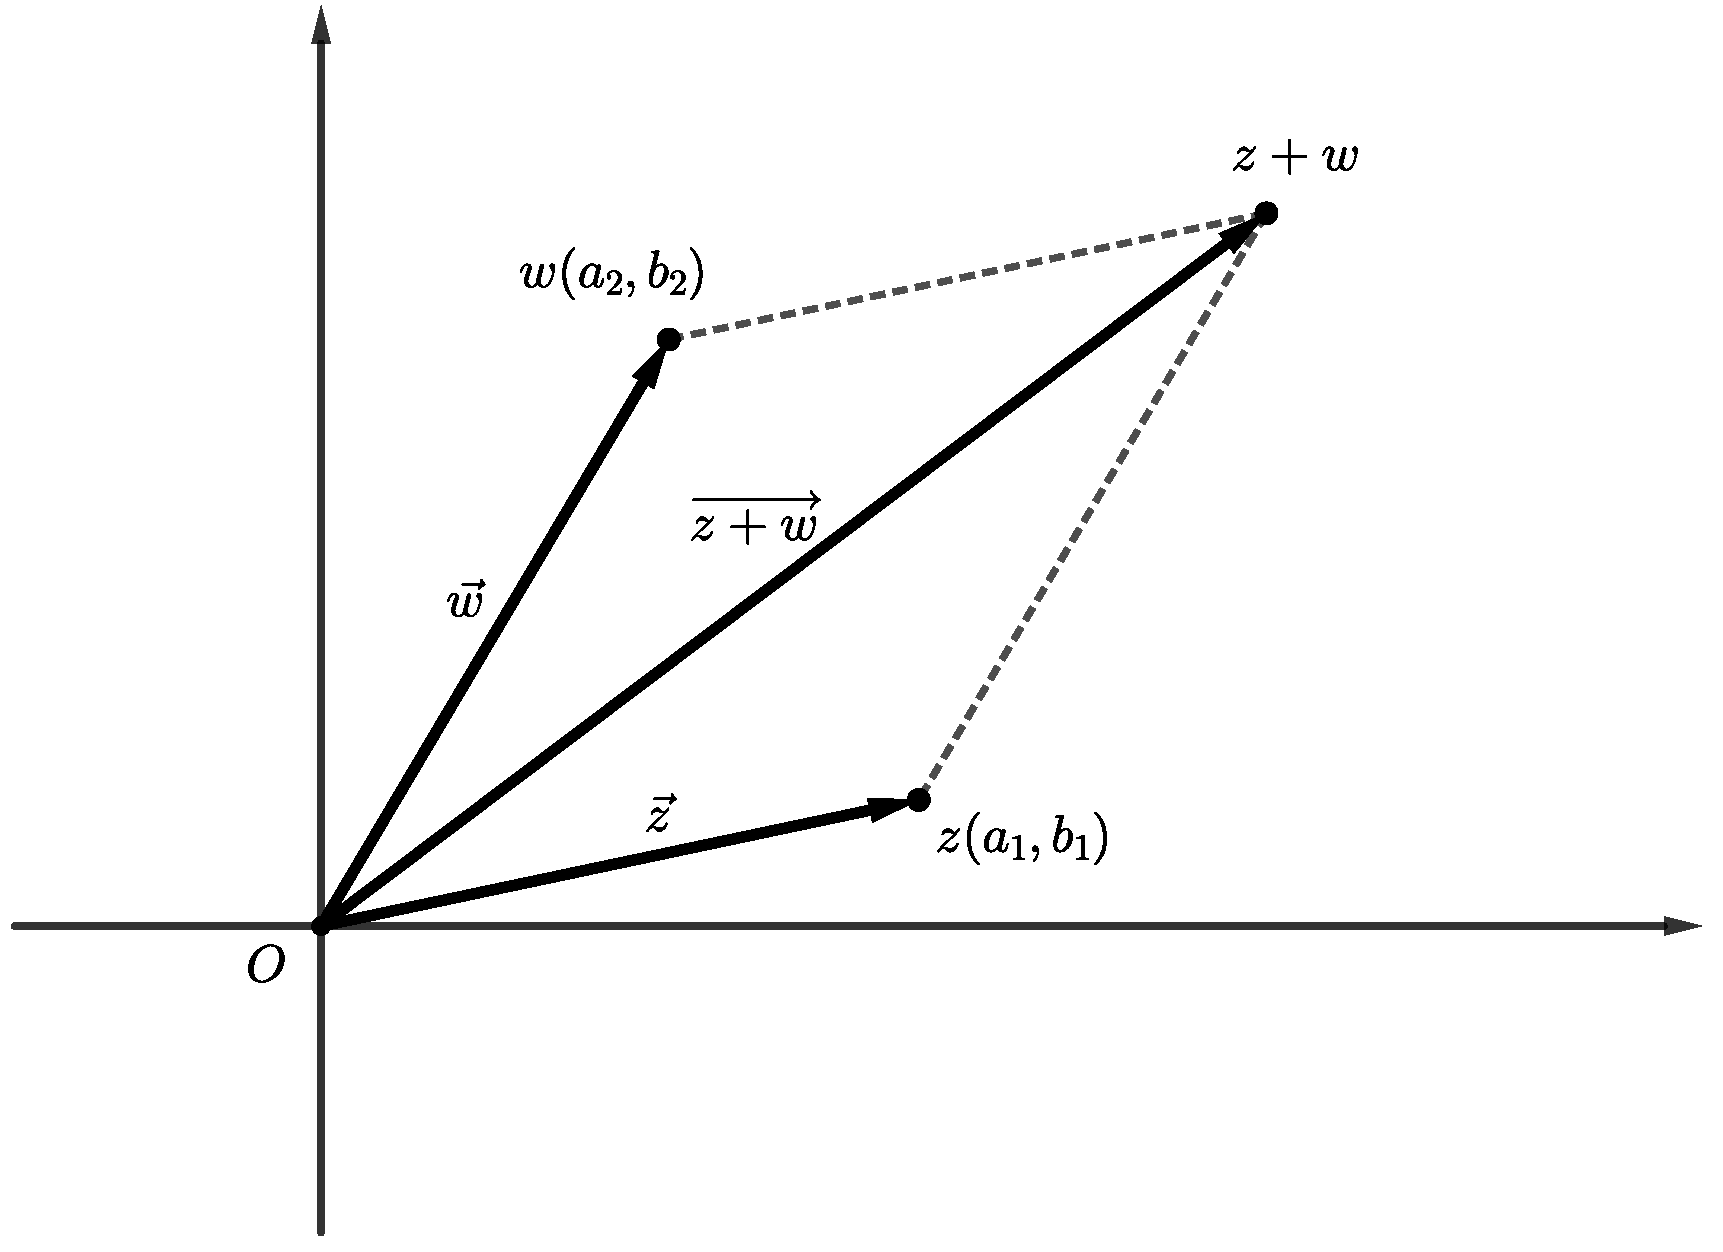
\includegraphics[width=0.7\textwidth]{grafici/complessi1}
	\caption{Due numeri complessi e la loro somma rappresentati nel piano di Argand-Gauss.}
	\label{compl:fig1}
\end{figure}


\subsection{Notazione trigonometrica}
I numeri complessi possono essere espressi in una forma, detta trigonometrica, la quale, pur essendo equivalente alla forma algebrica\footnote{Basti pensare che $\rho\cos\theta$ e $\rho\sin\theta$ sono le componenti del vettore $\vec z$}, possiede delle comode proprietà grafiche in riferimento al piano di Argand-Gauss:
\begin{equation}
	\label{compl:trigo}
	z=\rho(\cos\theta+i\sin{\theta})
\end{equation}
Dove $\rho$ indica il modulo $\abs{z}$ e $\theta$ l'argomento di $z$, ossia l'angolo che il vettore $\vec z$ forma con l'asse dei reali.

\begin{figure}[ht]
	\centering
	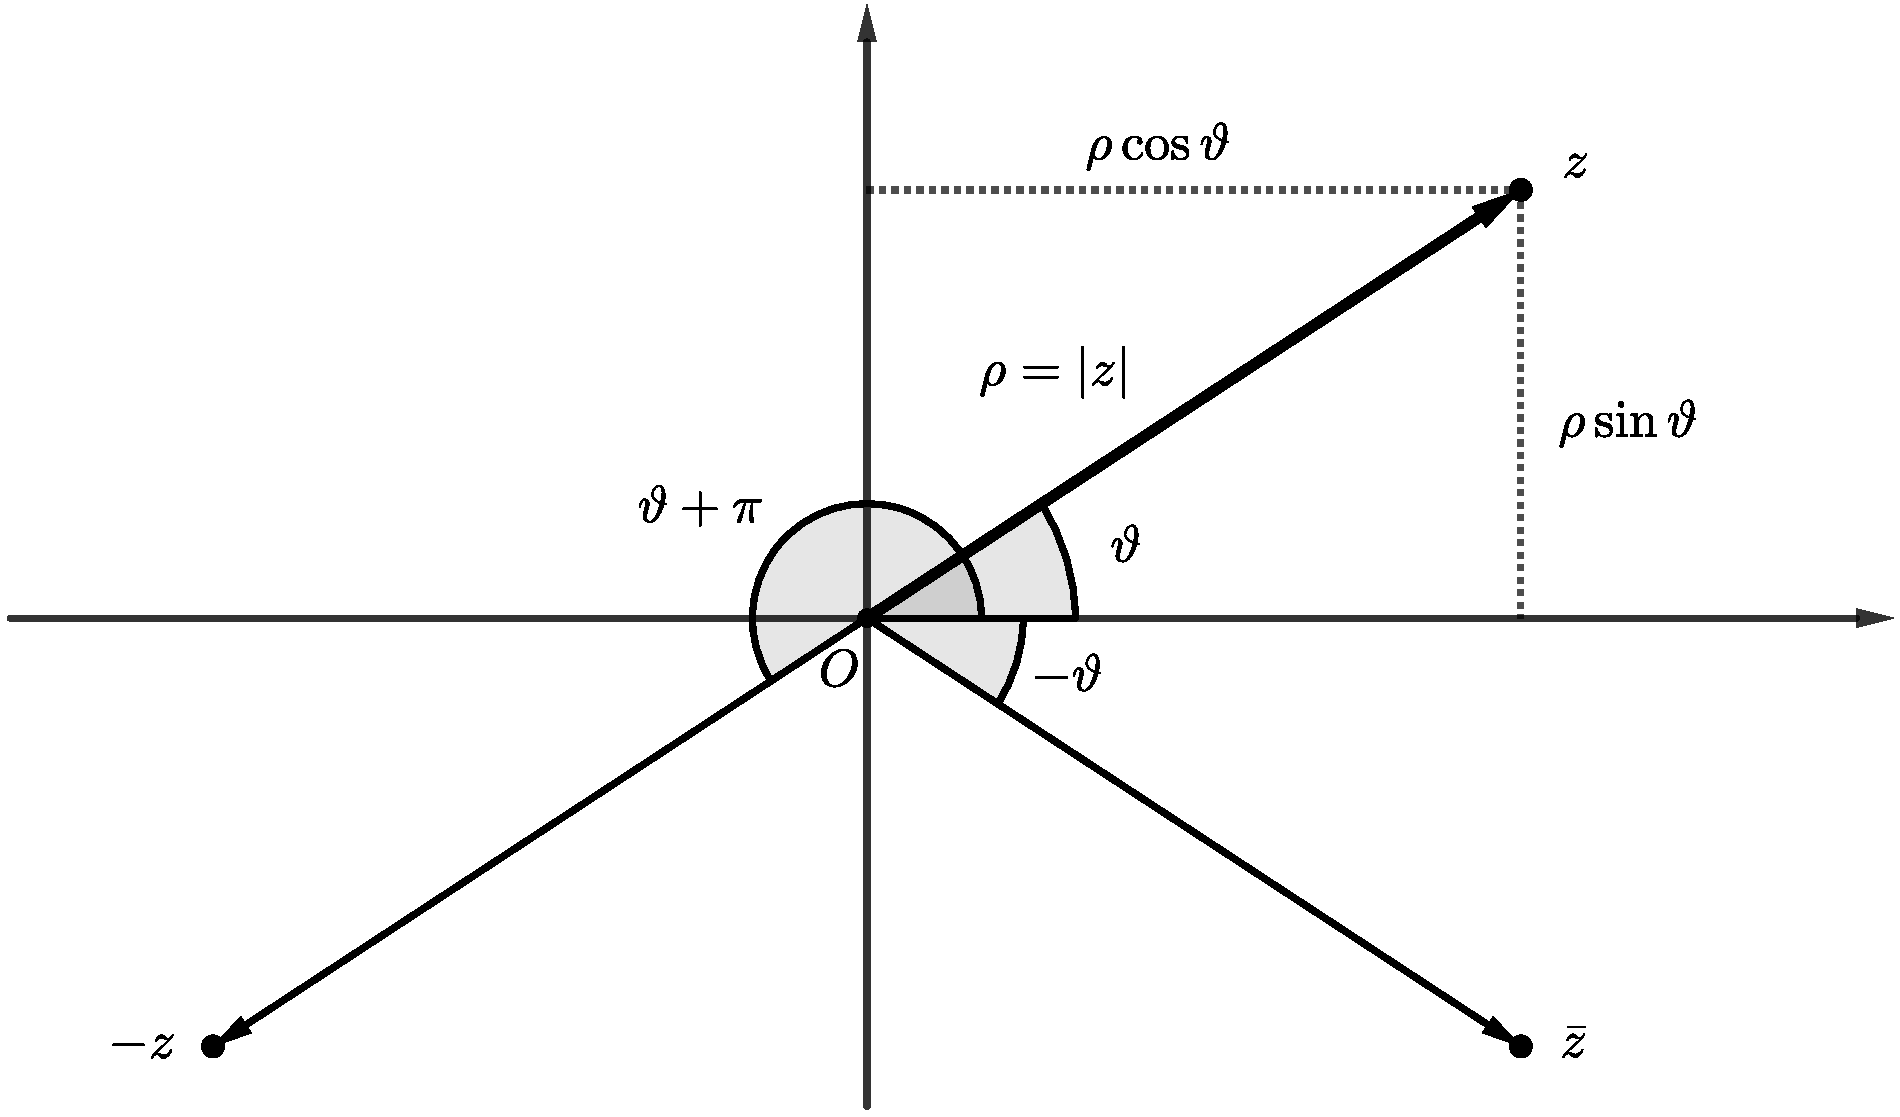
\includegraphics[width=0.9\textwidth]{grafici/complessi2b}
	\caption{Il numero complesso $z$, i suoi opposto e coniugato e i relativi parametri trigonometrici nel piano di Argand-Gauss}
	\label{compl:fig2}
\end{figure}

\subsubsection{Operazioni in forma trigonometrica}
In questo contesto due numeri complessi $z_1=\rho(\cos\theta+i\sin\theta)$ e $z_2=\sigma(\cos\varphi+i\sin\varphi)$ sono uguali se
\[
	\begin{cases}
		\rho=\sigma \\
		\theta=\varphi+2k\pi\qquad\text{con }k\in\Z
	\end{cases}
\]

Si possono facilmente esprimere alcune operazioni tra complessi in forma trigonometrica:
\begin{gather*}
	z_1\cdot z_2=\rho(\cos\theta+i\sin{\theta})\sigma(\cos\varphi+i\sin{\varphi})=\\
	\rho\sigma(\cos\theta\cos\varphi-\sin\theta\sin\varphi+i(\cos\theta\sin\varphi+\sin\theta\sin\varphi))=\\
	\rho\sigma(\cos(\theta+\varphi)+i\sin(\theta+\varphi))
\end{gather*}
Il prodotto di due numeri complessi in forma trigonometrica è un numero complesso che ha per modulo il prodotto dei moduli e per argomento la somma degli angoli. Geometricamente, avviene una dilatazione (o compressione) della distanza dall'origine e una rotazione rispetto agli assi. È facile dunque definire la potenza come moltiplicazione ripetuta:
\[
	z^n=\rho^n(\cos(n\theta)+i\sin(n\theta))
\]
E la potenza a esponente negativo come una potenza del reciproco:
\[
	z^{-n}=\frac{1}{\rho^{n}}(\cos(-n\theta)+i\sin(-n\theta))
\]

Alcuni numeri complessi notevoli in riferimento a $z$ così come espresso nella forma \ref{compl:trigo} (figura \vref{compl:fig2}):
\begin{align*}
	\bullet~ & -z=\rho(\cos(\theta+\pi)+i\sin(\theta+\pi))                                  \\
	\bullet~ & \bar z=\rho(\cos(-\theta)+i\sin(-\theta))                                    \\
	\bullet~ & z^{-1}=\frac{\bar z}{\abs{z}^2}=\frac{1}{\rho}(\cos(-\theta)+i\sin(-\theta))
\end{align*}

